\documentclass[border=2mm]{standalone}

\usepackage{pgfplots}
\pgfplotsset{compat=1.18}
\usetikzlibrary{arrows.meta, 
  calc, 
  positioning, 
  decorations.pathreplacing, 
  calligraphy}

\usepackage{xcolor}
\definecolor{den-1}{HTML}{111111}   % Đen #111111
\definecolor{den-2}{HTML}{222222}   % Đen #222222
\definecolor{den-3}{HTML}{333333}   % Đen #333333
\definecolor{den-4}{HTML}{444444}   % Đen #444444
\definecolor{den-5}{HTML}{555555}   % Đen #555555
\definecolor{den-6}{HTML}{666666}   % Đen #666666

\tikzset{
  >=Stealth,
  originlabel/.style={
    font=\small\sf,
    anchor=north east, 
    yshift=-0.1ex,     
    xshift=-0.1ex      
  }
}

\begin{document}

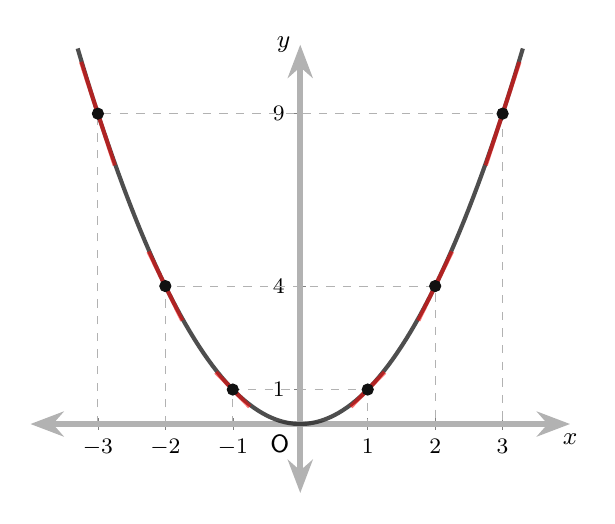
\begin{tikzpicture}

\begin{axis}[
    font=\small\sf,
    axis lines=middle,axis line style={<->, line width=2pt, den-6!50},
    xlabel=$x$, ylabel=$y$,
    xlabel style={below, font=\small\sf},
    ylabel style={left, font=\small\sf},
    xmin=-4, xmax=4,
    ymin=-2, ymax=11,
    xtick={-3,-2,-1,0,1,2,3},
    ytick={0,1,4,9},
    tick label style={font=\footnotesize\sf},
    clip=false,
]

\node[originlabel] at (axis cs:0,0) {O};

\draw [dashed, color=den-6!50] (-1,0) -- (-1,1) -- (1,1) -- (1,0);
\draw [dashed, color=den-6!50] (-2,0) -- (-2,4) -- (2,4) -- (2,0);
\draw [dashed, color=den-6!50] (-3,0) -- (-3,9) -- (3,9) -- (3,0);

\addplot[domain=-3.3:3.3, samples=100, line width=1.5pt, color=den-2, opacity=.8] 
    {x^2};

\foreach \x in {-3,-2,-1,1,2,3} 
{
    \addplot[only marks, mark=*, mark size=2pt, color=den-1] 
        coordinates {(\x,{(\x)^2})};
}

% Vẽ tiếp tuyến
\addplot[red, opacity=.55, line width=1.5pt, domain=-1.25:-.75] {-2*x - 1};
\addplot[red, opacity=.55, line width=1.5pt, domain=-2.25:-1.75] {-4*x - 4};
\addplot[red, opacity=.55, line width=1.5pt, domain=-3.25:-2.75] {-6*x - 9};

\addplot[red, opacity=.55, line width=1.5pt, domain=.75:1.25] {2*x - 1};
\addplot[red, opacity=.55, line width=1.5pt, domain=1.75:2.25] {4*x - 4};
\addplot[red, opacity=.55, line width=1.5pt, domain=2.75:3.25] {6*x - 9};

\end{axis}

\end{tikzpicture}

\end{document}
